% Capítulo 4
\chapter{Resultados}
\label{resultados}

Para cada um dos anos eleitorais analisados neste estudo são apresentados duas visualizações para o grafo de cada ano. Na primeira é possível identificar as comunidades encontradas pelo algoritmo de modularização, de maneira que cada comunidade possui uma cor diferente para seus vértices. Na segunda visualização do grafo cada vértice é colorido de acordo com a afinidade ideológica do partido.

Vértices em tons de vermelho são partidos de centro-esquerda, esquerda e extrema-esquerda. Vértices em tons de azul são partidos de centro-direita, direita e extrema-direita. Já os vértices verdes são os partidos que se declaram de centro, e os cinzas são partidos que não possuem uma classificação bem definida na literatura.

%%%%%%%%%%%%%%%%%%%%%%%%%%%%%%%%%%%%%%%%%%%%%%%%%%%%%%%%%%%
\section{\texorpdfstring{\MakeUppercase{Métricas de avaliação}}{}}
\label{resultados__metricas-avaliacao}

Como visto na sessão \ref{proposta__modelagem}, utilizamos pesos nas arestas dos grafos como forma de indicar em quantos estados dois determinados partidos fazem coligação. Assim, os grafos apresentados não indicam apenas quais são as alianças formadas, mas também o quão forte é um relacionamento entre dois partidos.

%%%%%%%%%%%%%%%%%%%%%%%%%%%%%%%%%%%%%%%%%%%%%%%%%%%%%%%%%%%
\section{\texorpdfstring{\MakeUppercase{Parâmetros para modularização}}{}}
\label{resultados__parametros-modularizacao}

Para a utilização do algoritmo de detecção de comunidades é necessário escolher um parâmetro de \emph{resolução}, quanto maior o valor deste parâmetro menos comunidades são geradas.

Assim, utilizamos o valor de resolução 1.2 para os grafos de 1994, 1998, 2002 e 2006. Com este parâmetro, o algoritmo de modularização conseguiu separar a componente gigante dos grafos em duas comunidades. Para os anos 2010 e 2014 percebeu-se a necessidade de reduzir o valor de resolução para 1.0, uma vez que ao utilizar 1.2 como parâmetro a componente gigante se tornava uma única comunidade (mais detalhes em \nameref{resultados__grafos--2010} e \ref{resultados__grafos--2014}).

%%%%%%%%%%%%%%%%%%%%%%%%%%%%%%%%%%%%%%%%%%%%%%%%%%%%%%%%%%%
\section{\texorpdfstring{\MakeUppercase{Grafos}}{}}
\label{resultados__grafos}
%% Gráficos, números, conclusões: como as comunidades ficaram, grau médio, coeficiente de clustering


\subsection{1994}
\label{resultados__grafos--1994}

\begin{figure}[H]
\center
    \subfigure[fig-1994][Comunidades identificadas]{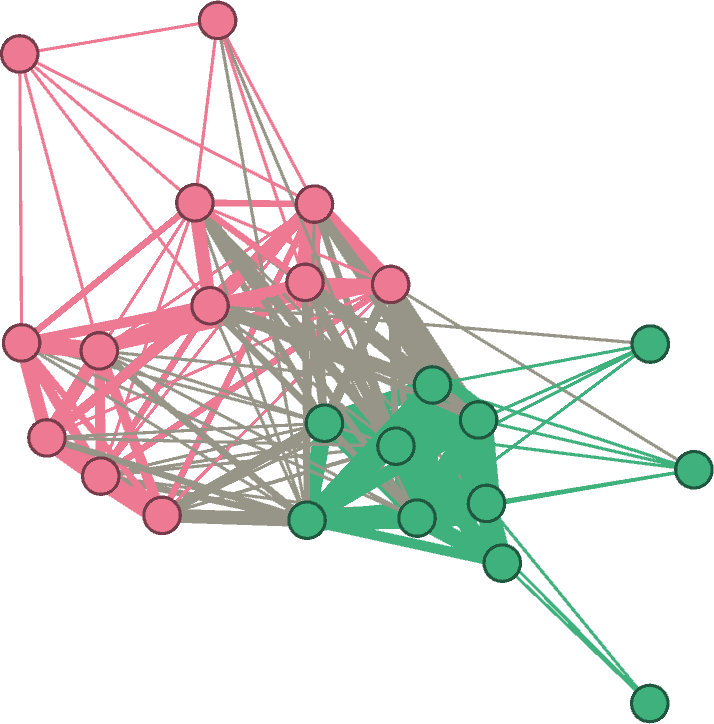
\includegraphics[width=7.5cm]{img/grafos/1994a.png}}
    \qquad
    \subfigure[fig-1994b][Espectro político dos partidos]{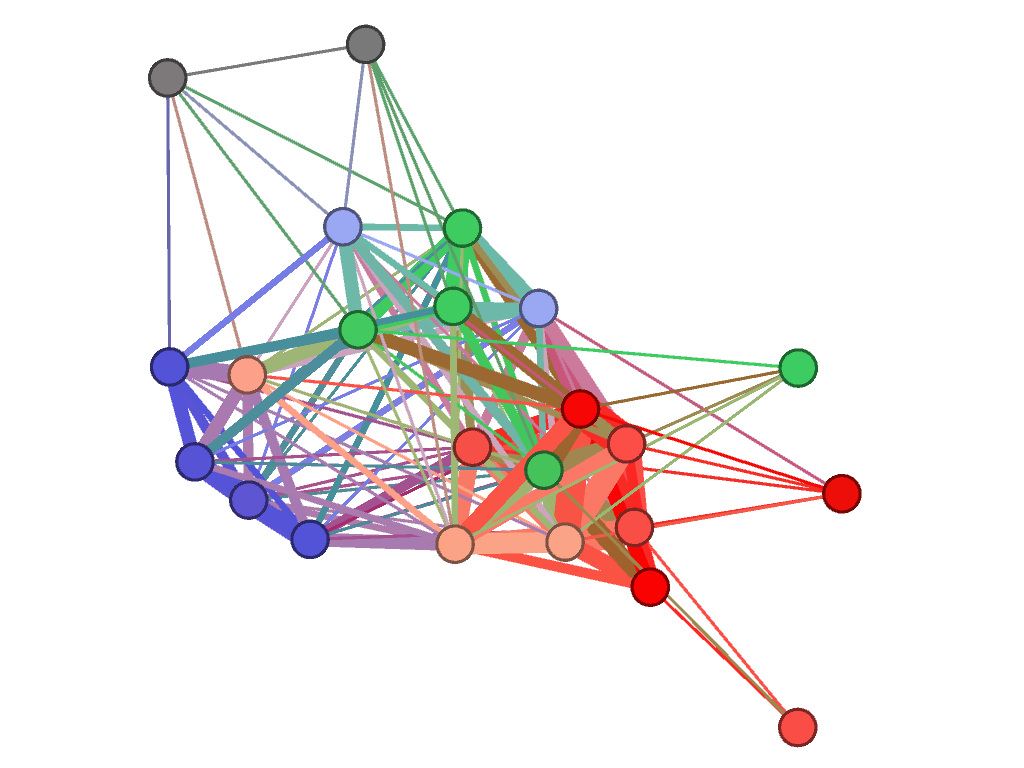
\includegraphics[width=7.5cm]{img/grafos/1994c.png}}

    \caption{1994: Comunidades e espectro político}
\end{figure}

Ao comparar as duas visualizações do grafo de 1994 nota-se uma divisão evidente na afinidade ideológica predominante em cada comunidade. A comunidade identificada pela cor verde contém 11 partidos, dos quais 8 são de esquerda e 2 são de centro. A comunidade rosa apresenta 12 partidos, 6 deles são de direita e 3 de centro.

Ressalta-se que esta separação não significa que partidos da esquerda só fazem aliança com partidos de ideologia parecida por exemplo. As arestas dos grafos tendem a manter a cor dos vértices em que elas incidem, e no grafo (a) podemos ver uma grande quantidade de arestas cinzas, que apresentam esta cor por conectar vértices rosas e verdes. Isto significa que existem várias alianças sendo feitas entre os partidos das duas comunidades opostas.

Percebe-se ainda que os partidos sem classificação ideológica (\gls{PRN} e \gls{PTRB}, vértices cinzas) ficaram nas bordas do grafo, indicando que possuem grau menor em relação aos demais vértices e, portanto, fizeram menos alianças, assim como os vértices nas extremidades da comunidade verde (\gls{PCB}, \gls{PTdoB} e \gls{PRONA}).


\subsection{1998}
\label{resultados__grafos--1998}

\begin{figure}[H]
\center
    \subfigure[fig-1998][Comunidades identificadas]{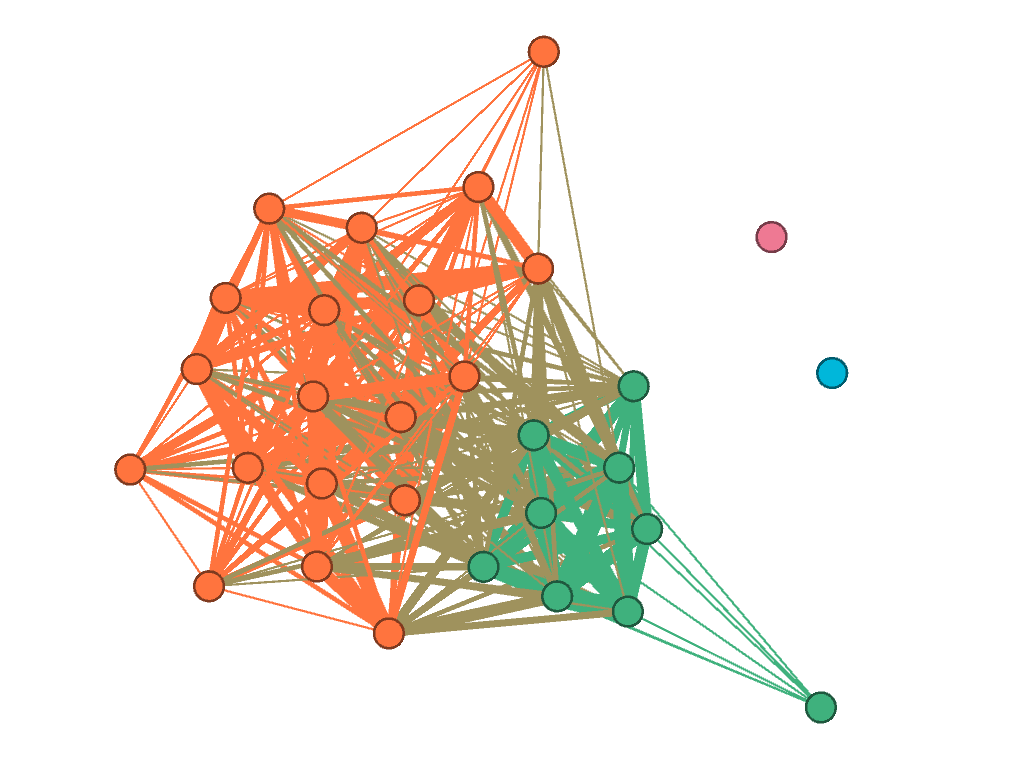
\includegraphics[width=7.5cm]{img/grafos/1998a.png}}
    \qquad
    \subfigure[fig-1998b][Espectro político dos partidos]{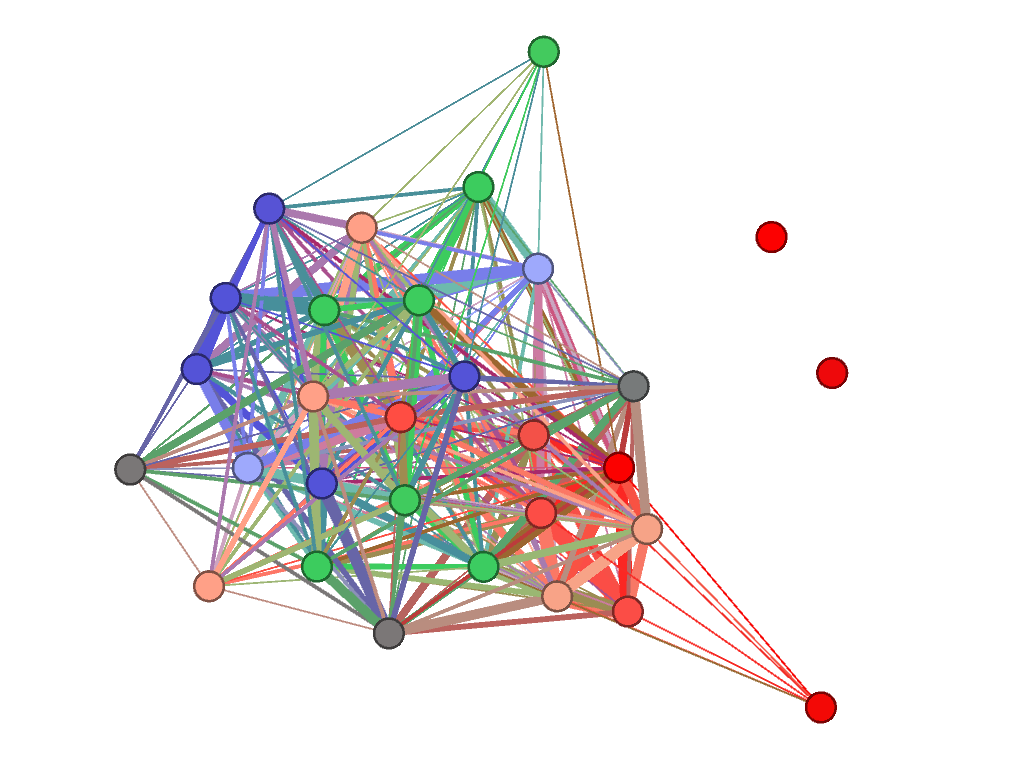
\includegraphics[width=7.5cm]{img/grafos/1998c.png}}

    \caption{1998: Comunidades e espectro político}
\end{figure}

Percebe-se que o grafo gerado para 1998 não é conexo, contendo dois vértices sem arestas. Isso indica que existem dois partidos que não se coligaram em nenhum estado do Brasil nesse ano (\gls{PCO} e \gls{PSTU}). Estes vértices não são considerados comunidades propriamente ditas, mas optamos por manter no grafo para uma melhor visualização do comportamento geral de todos os partidos.

A divisão dos partidos de esquerda e direita nas duas comunidades manteve-se neste ano, apesar de não ser tão clara quanto em 1994. Isso se dá, em parte, ao fato de que as duas comunidades são mais densas e o grafo possui mais vértices.

É possível observar ainda três partidos de centro-esquerda e um de esquerda na comunidade com predominância de partidos de direita: \gls{PTdoB}, \gls{PGT}, \gls{PTB} e \gls{PST}.
- dentre os 7 partidos de centro, apenas um ficou no cluster de esquerda
- os dois cinzas vieram para mais ao centro do grafo, o q significa q fizeram muito mais alianças

\subsection{2002}
\label{resultados__grafos--2002}

\begin{figure}[H]
\center
    \subfigure[fig-2002][Comunidades identificadas]{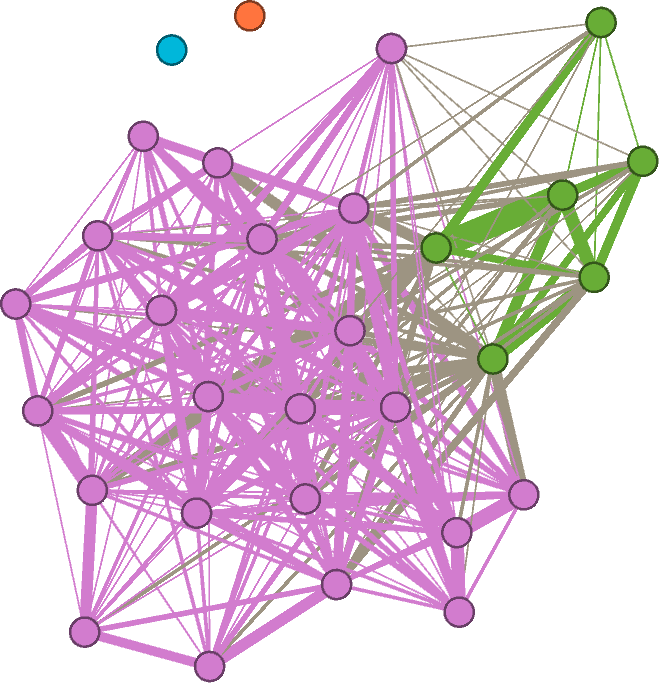
\includegraphics[width=7.5cm]{img/grafos/2002a.png}}
    \qquad
    \subfigure[fig-2002b][Espectro político dos partidos]{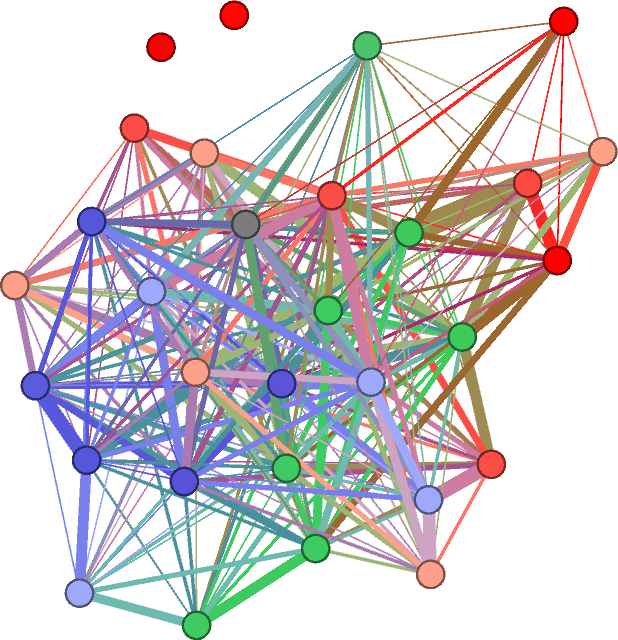
\includegraphics[width=7.5cm]{img/grafos/2002c.png}}

    \caption{comentario}
\end{figure}


\subsection{2006}
\label{resultados__grafos--2006}

\begin{figure}[H]
\center
    \subfigure[fig-2006][Comunidades identificadas]{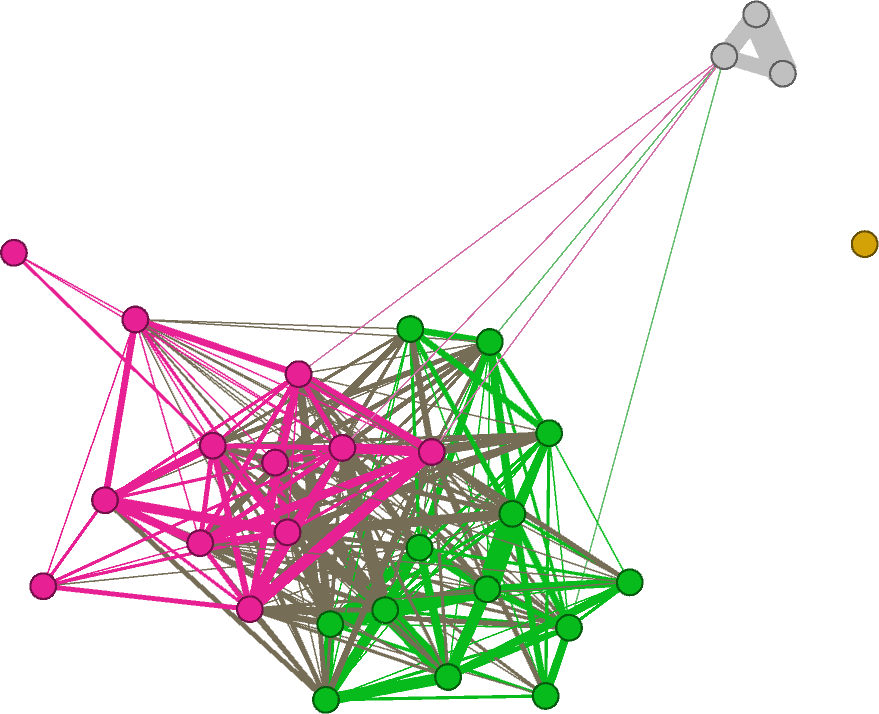
\includegraphics[width=7.5cm]{img/grafos/2006a.png}}
    \qquad
    \subfigure[fig-2006b][Espectro político dos partidos]{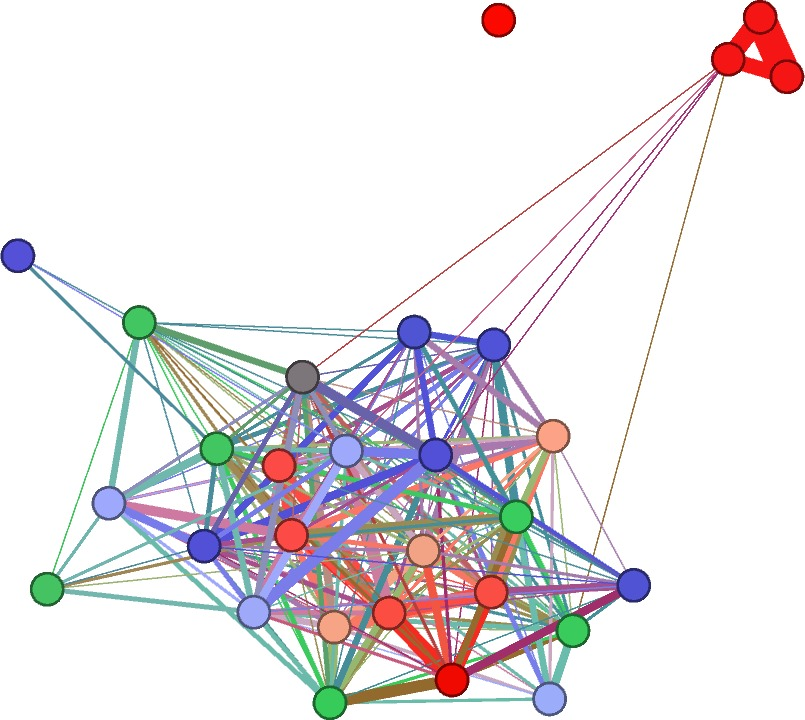
\includegraphics[width=7.5cm]{img/grafos/2006c.png}}

    \caption{comentario}
\end{figure}


\subsection{2010}
\label{resultados__grafos--2010}

\begin{figure}[H]
\center
    \subfigure[fig-2010][Comunidades identificadas]{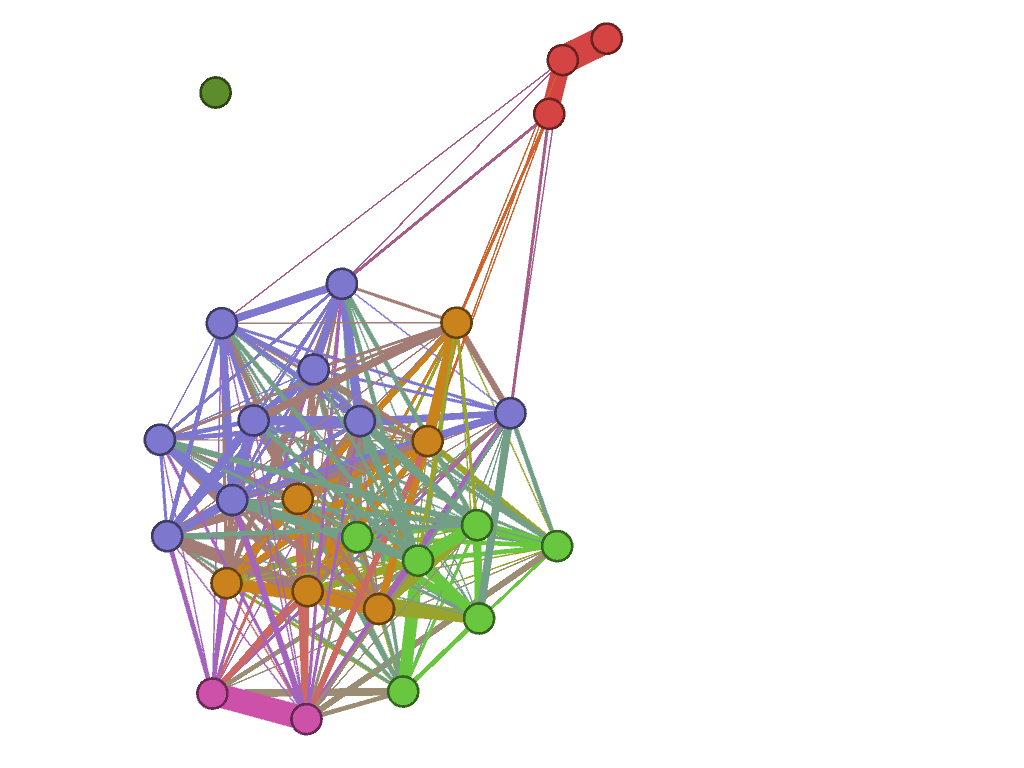
\includegraphics[width=7.5cm]{img/grafos/2010a.png}}
    \qquad
    \subfigure[fig-2010b][Espectro político dos partidos]{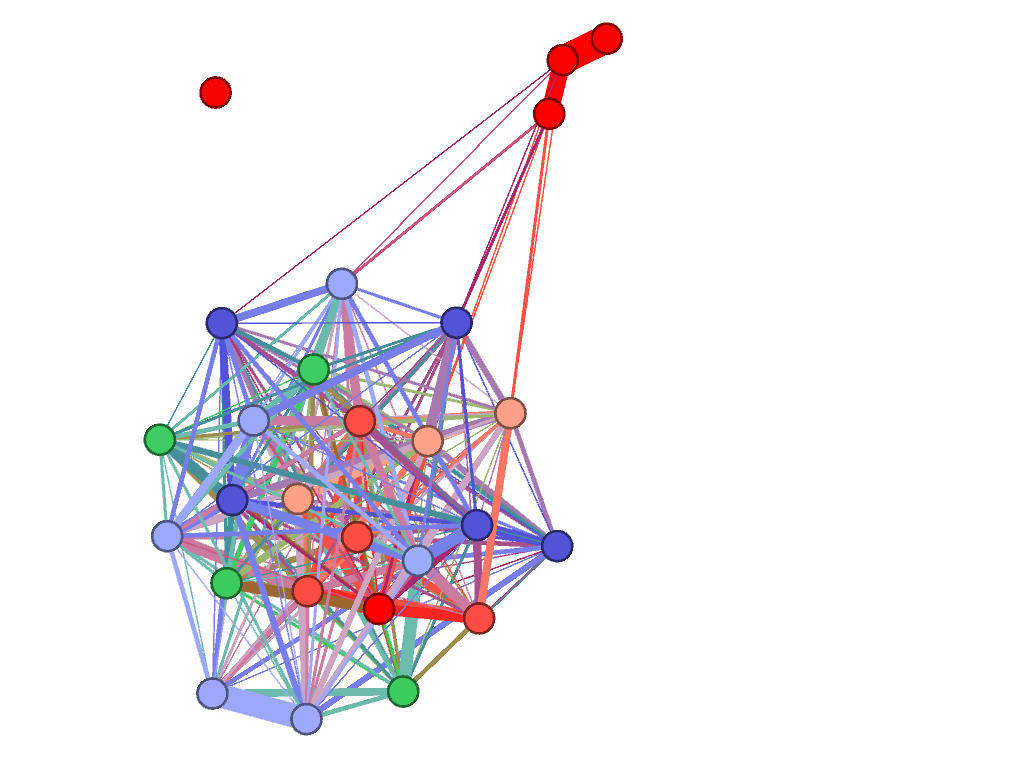
\includegraphics[width=7.5cm]{img/grafos/2010c.png}}

    \caption{comentario}
\end{figure}

\subsection{2014}
\label{resultados__grafos--2014}

\begin{figure}[H]
\center
    \subfigure[fig-2014][Comunidades identificadas]{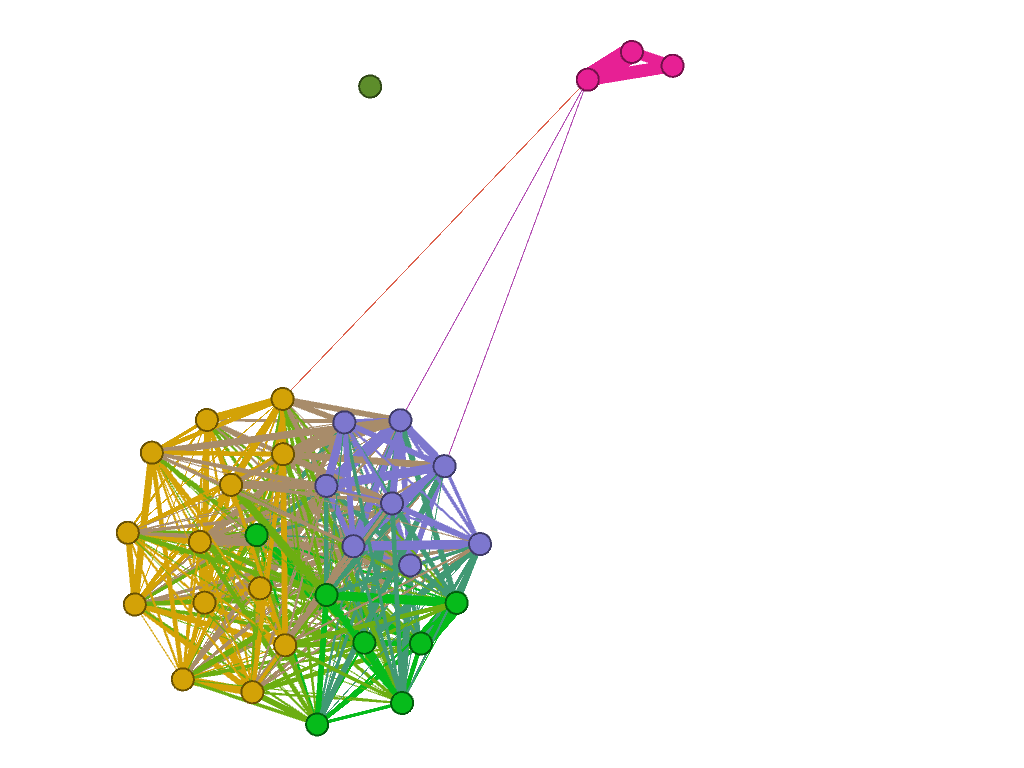
\includegraphics[width=7.5cm]{img/grafos/2014a.png}}
    \qquad
    \subfigure[fig-2014b][Espectro político dos partidos]{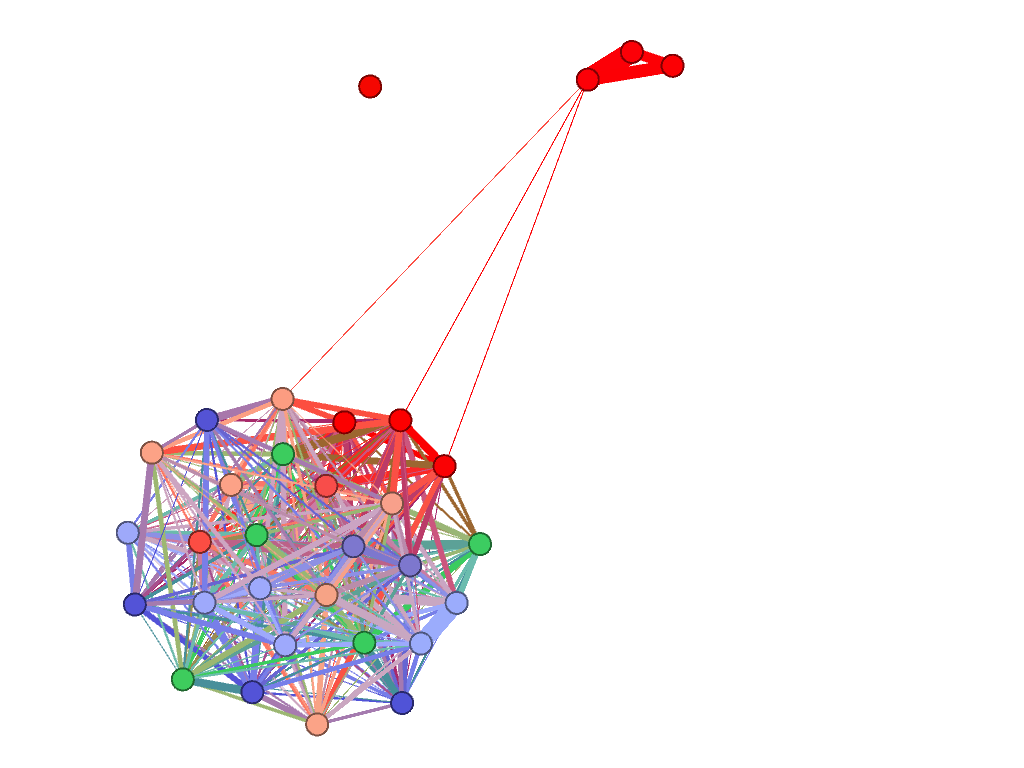
\includegraphics[width=7.5cm]{img/grafos/2014c.png}}

    \caption{comentario}
\end{figure}


%%%%%%%%%%%%%%%%%%%%%%%%%%%%%%%%%%%%%%%%%%%%%%%%%%%%%%%%%%%
\section{\texorpdfstring{\MakeUppercase{Conclusão geral}}{}}
\label{resultados__conclusao-geral}

Conclusão geral
